%Drafted by Anika Maria Athena R. Acosta

\documentclass[12pt,a4paper,twoside]{article}
\input{183.dat}
\usepackage{gensymb}
\usepackage{float}
\usepackage{siunitx}
\usepackage{amsmath}
\usepackage{physics}
\usepackage{listings}
\usepackage{enumerate}

\begin{document}

\begin{titlepage}
\begin{center}
\vspace*{\fill}

\Huge{ Behavior of 2\textsuperscript{nd} order underdamped system \\
6 March 2019
} \\

\qquad
\qquad

\normalsize{Kenneth V. Domingo \\
2015-03116
}

\vspace*{\fill}
\end{center}
\end{titlepage}

\setcounter{page}{1}

\begin{enumerate}[(1)]

\begin{figure}[!h]
	\centering
	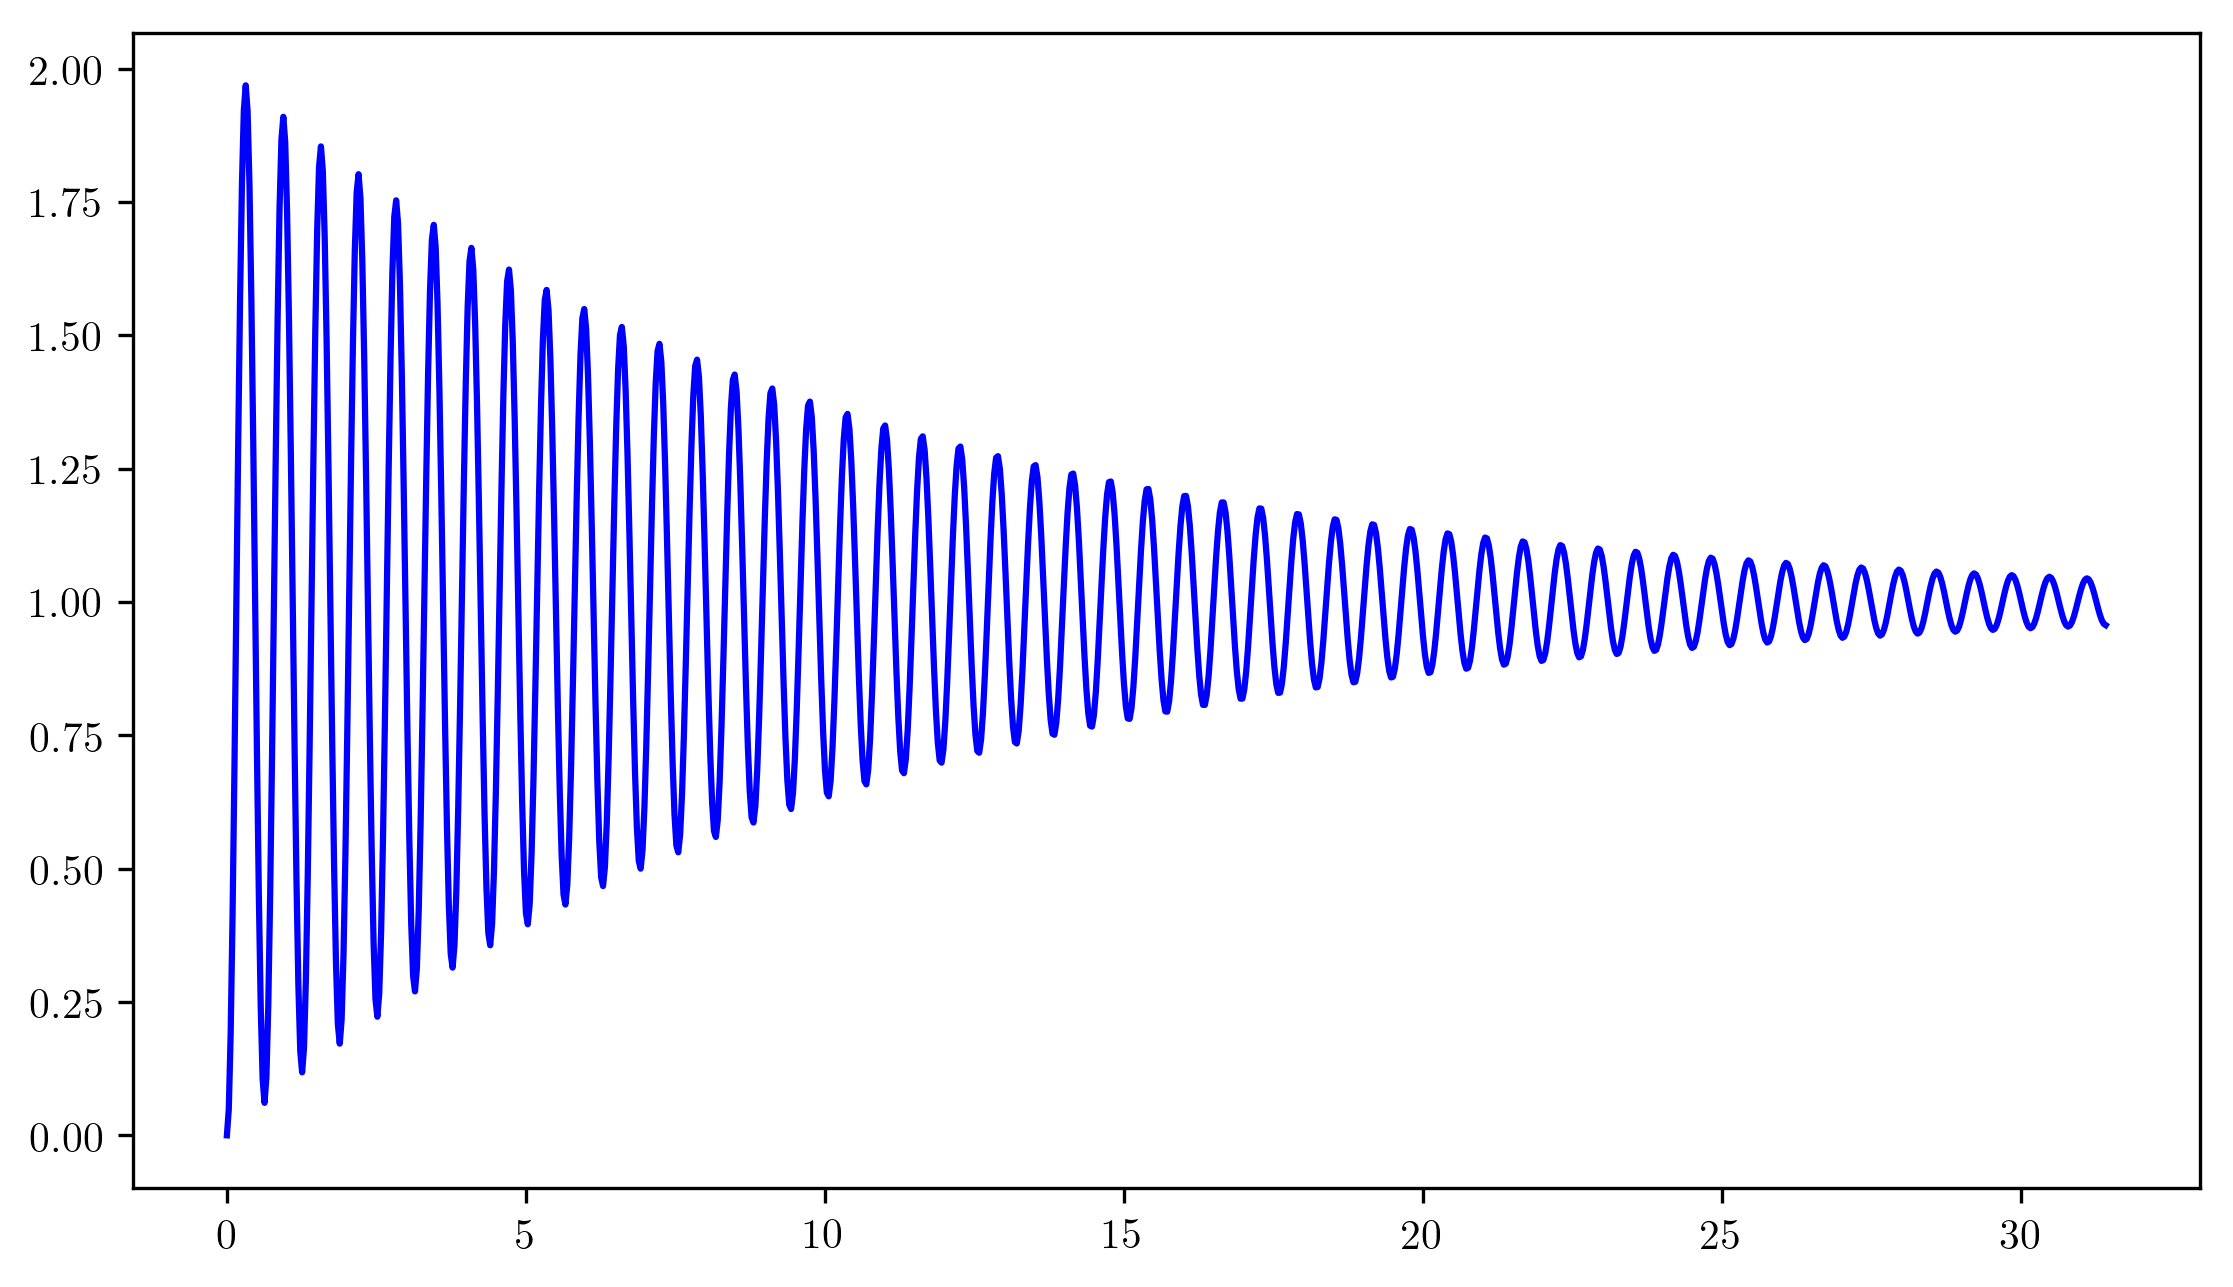
\includegraphics[width=\textwidth]{original.png}
	\caption{Original waveform, $\zeta = 0.01$, $\omega_n = 10$.}
	\label{fig:original}
\end{figure}

\clearpage
\item \textbf{Reduced real part}

\paragraph{Predict} Since the exponential (envelope) depends on the real part, decreasing it will further decrease the exponential term because of the negative sign already present. The envelope will therefore decay faster.

\begin{figure}[!h]
	\centering
	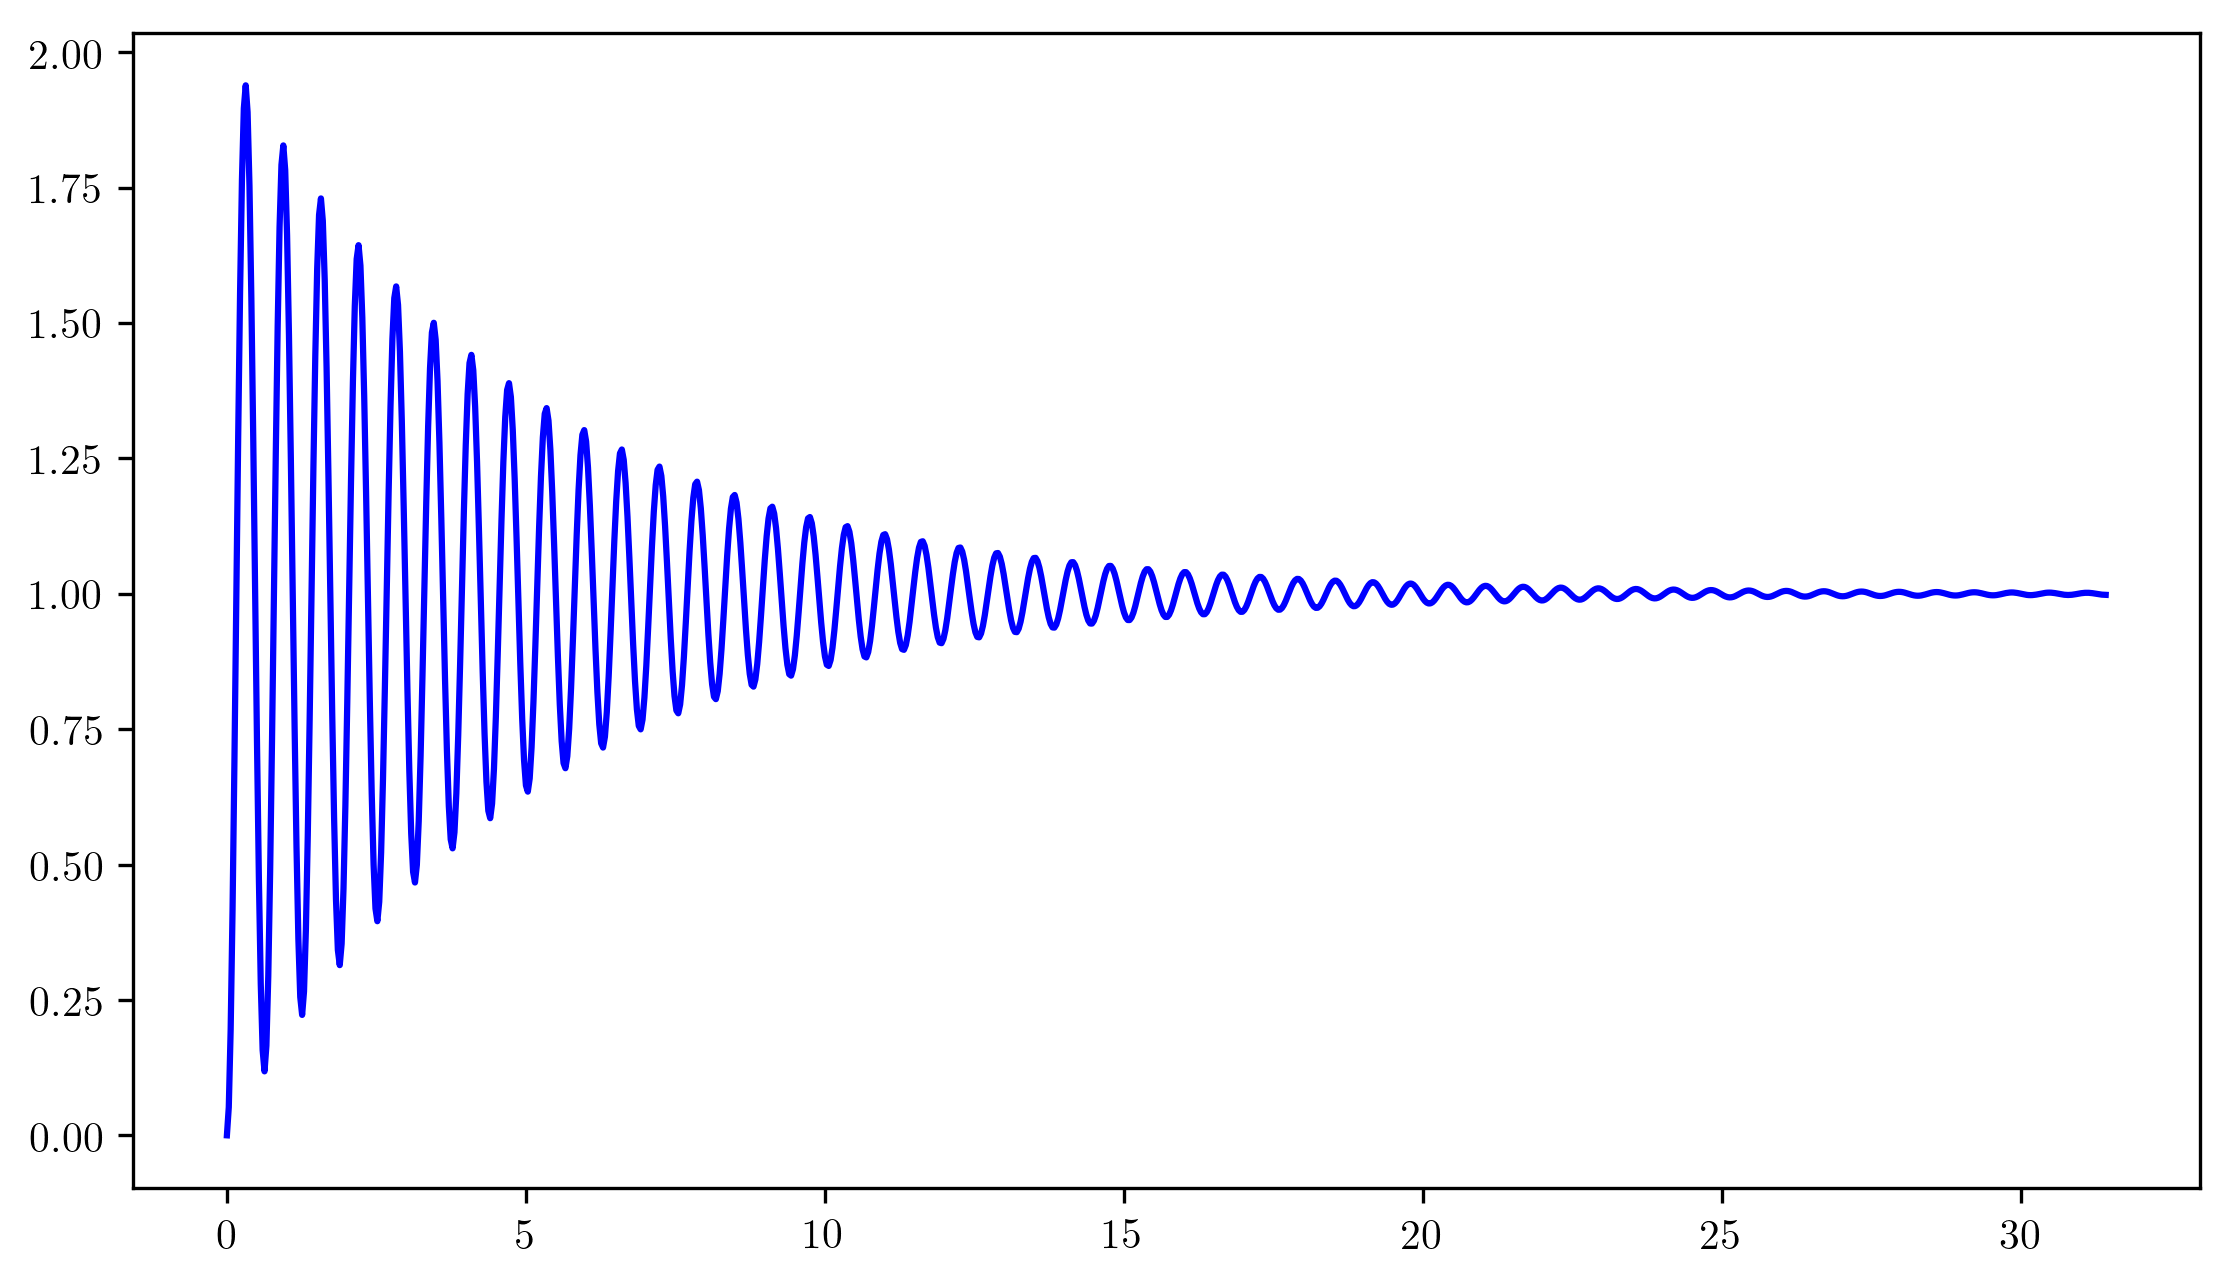
\includegraphics[width=\textwidth]{minusreal.png}
	\caption{$\Re[c(t)] - 0.1$.}
	\label{fig:minusreal}
\end{figure}

\paragraph{Explain} The observation agrees with the prediction.

\clearpage
\item \textbf{Wide imaginary part}

\paragraph{Predict} Since the cosine term depends on the imaginary part, which is dependent on the frequency. Since the frequencies are symmetric about zero in the frequency domain, we need only to consider the positive or absolute frequency. When the imaginary part is increased, the frequency also increases.

\begin{figure}[!h]
	\centering
	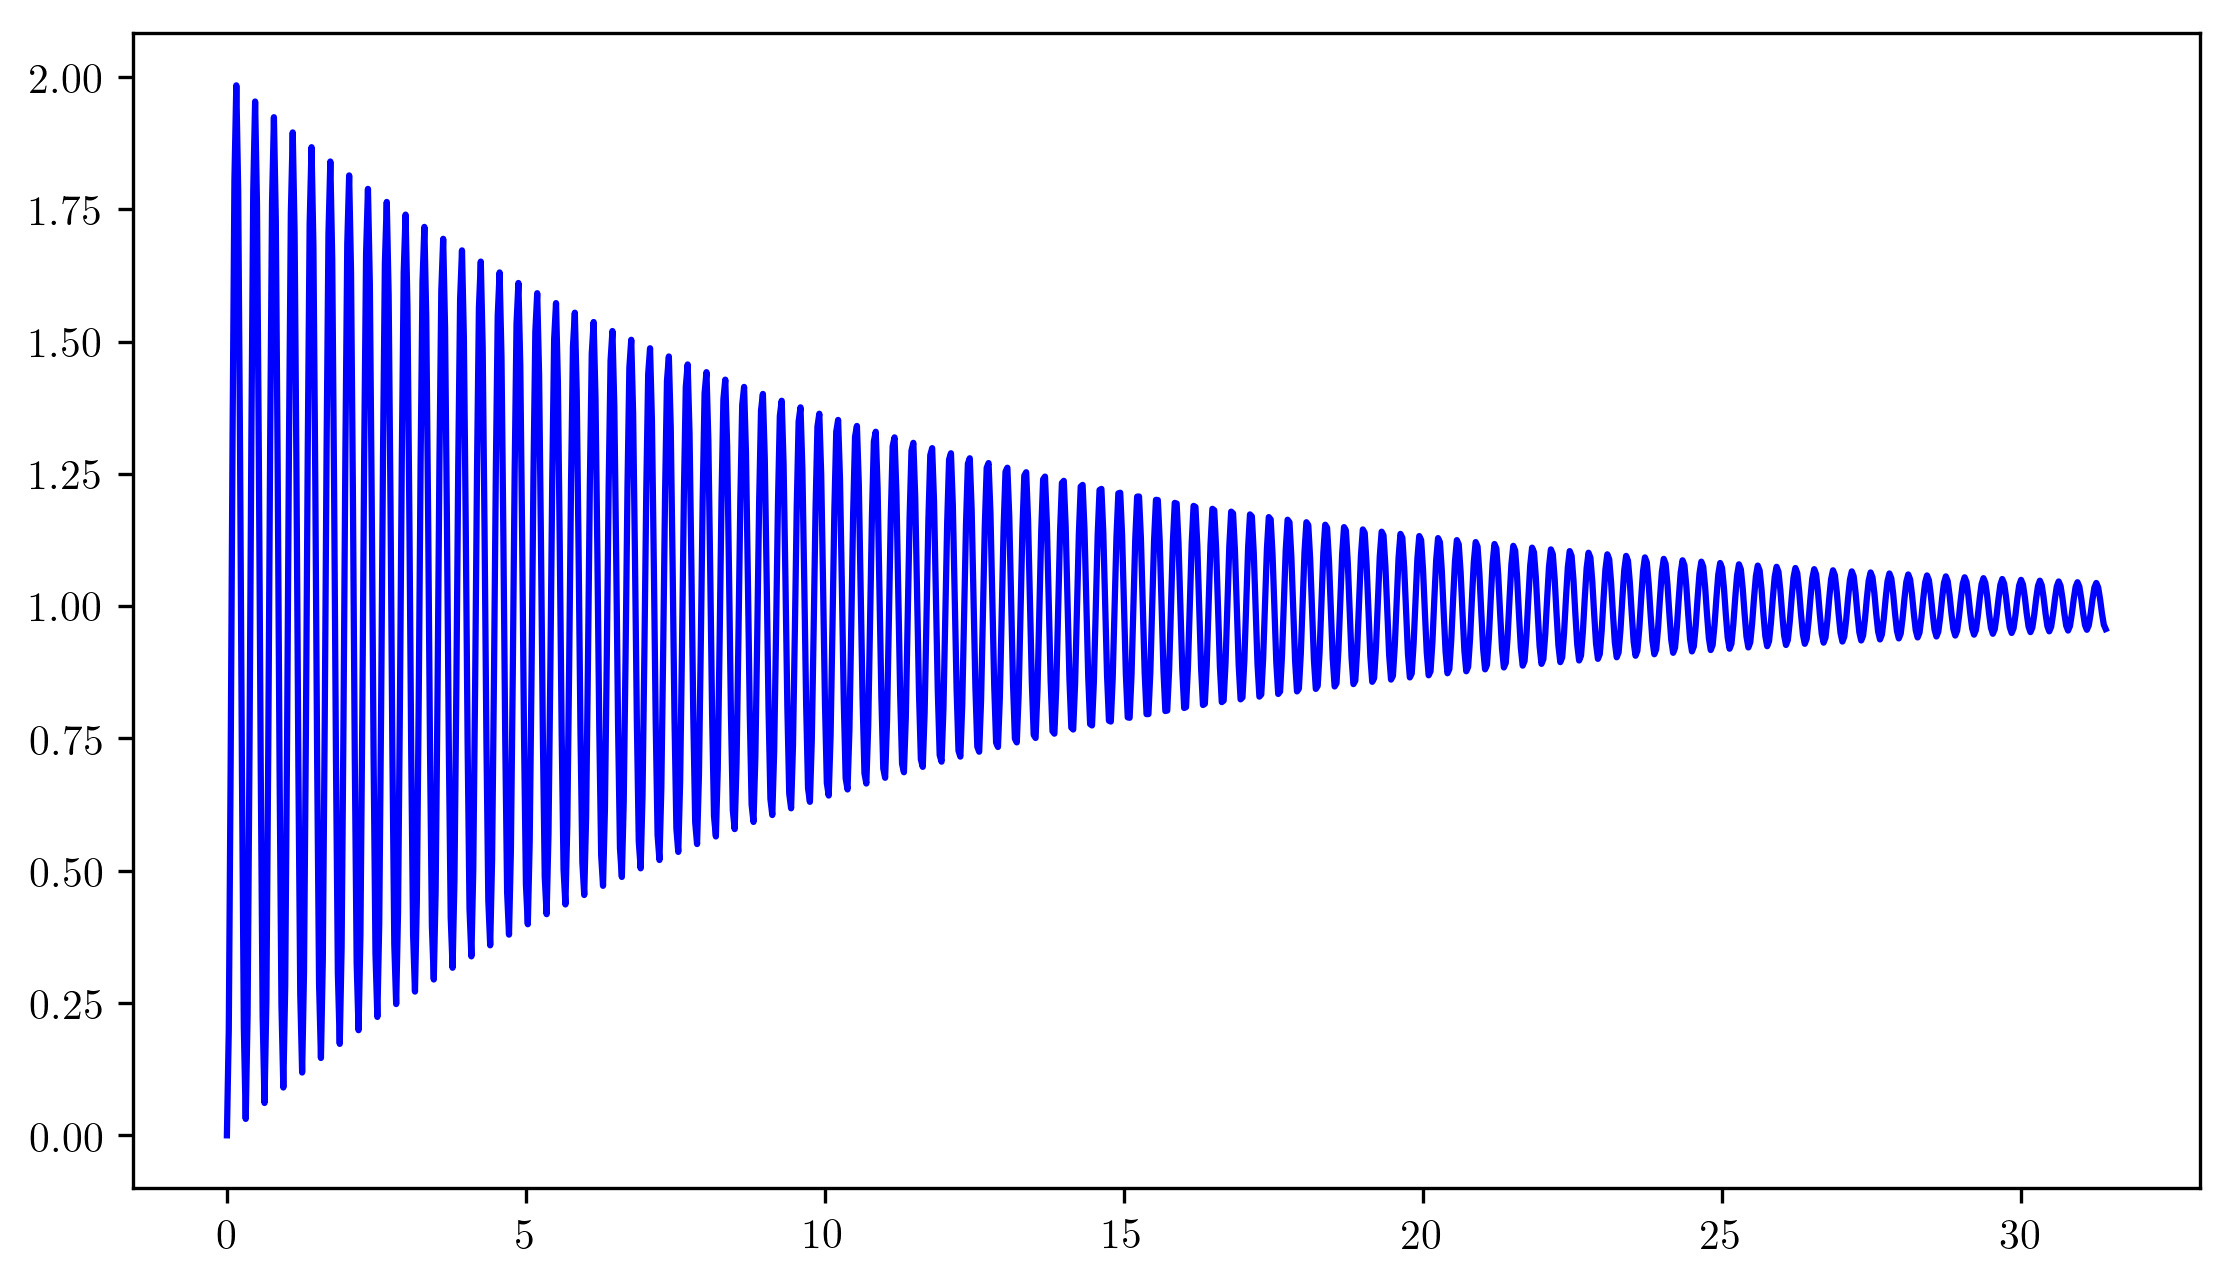
\includegraphics[width=\textwidth]{plusimag.png}
	\caption{$\Im[c(t)] - 10$.}
	\label{fig:plusimag}
\end{figure}

\paragraph{Explain} The observation agrees with the prediction.

\clearpage
\item \textbf{Increased angle}

\paragraph{Predict} The real part is decreased and the imaginary part is widened equally. Thus, the envelope will decay faster and the frequency will increase.

\begin{figure}[!h]
	\centering
	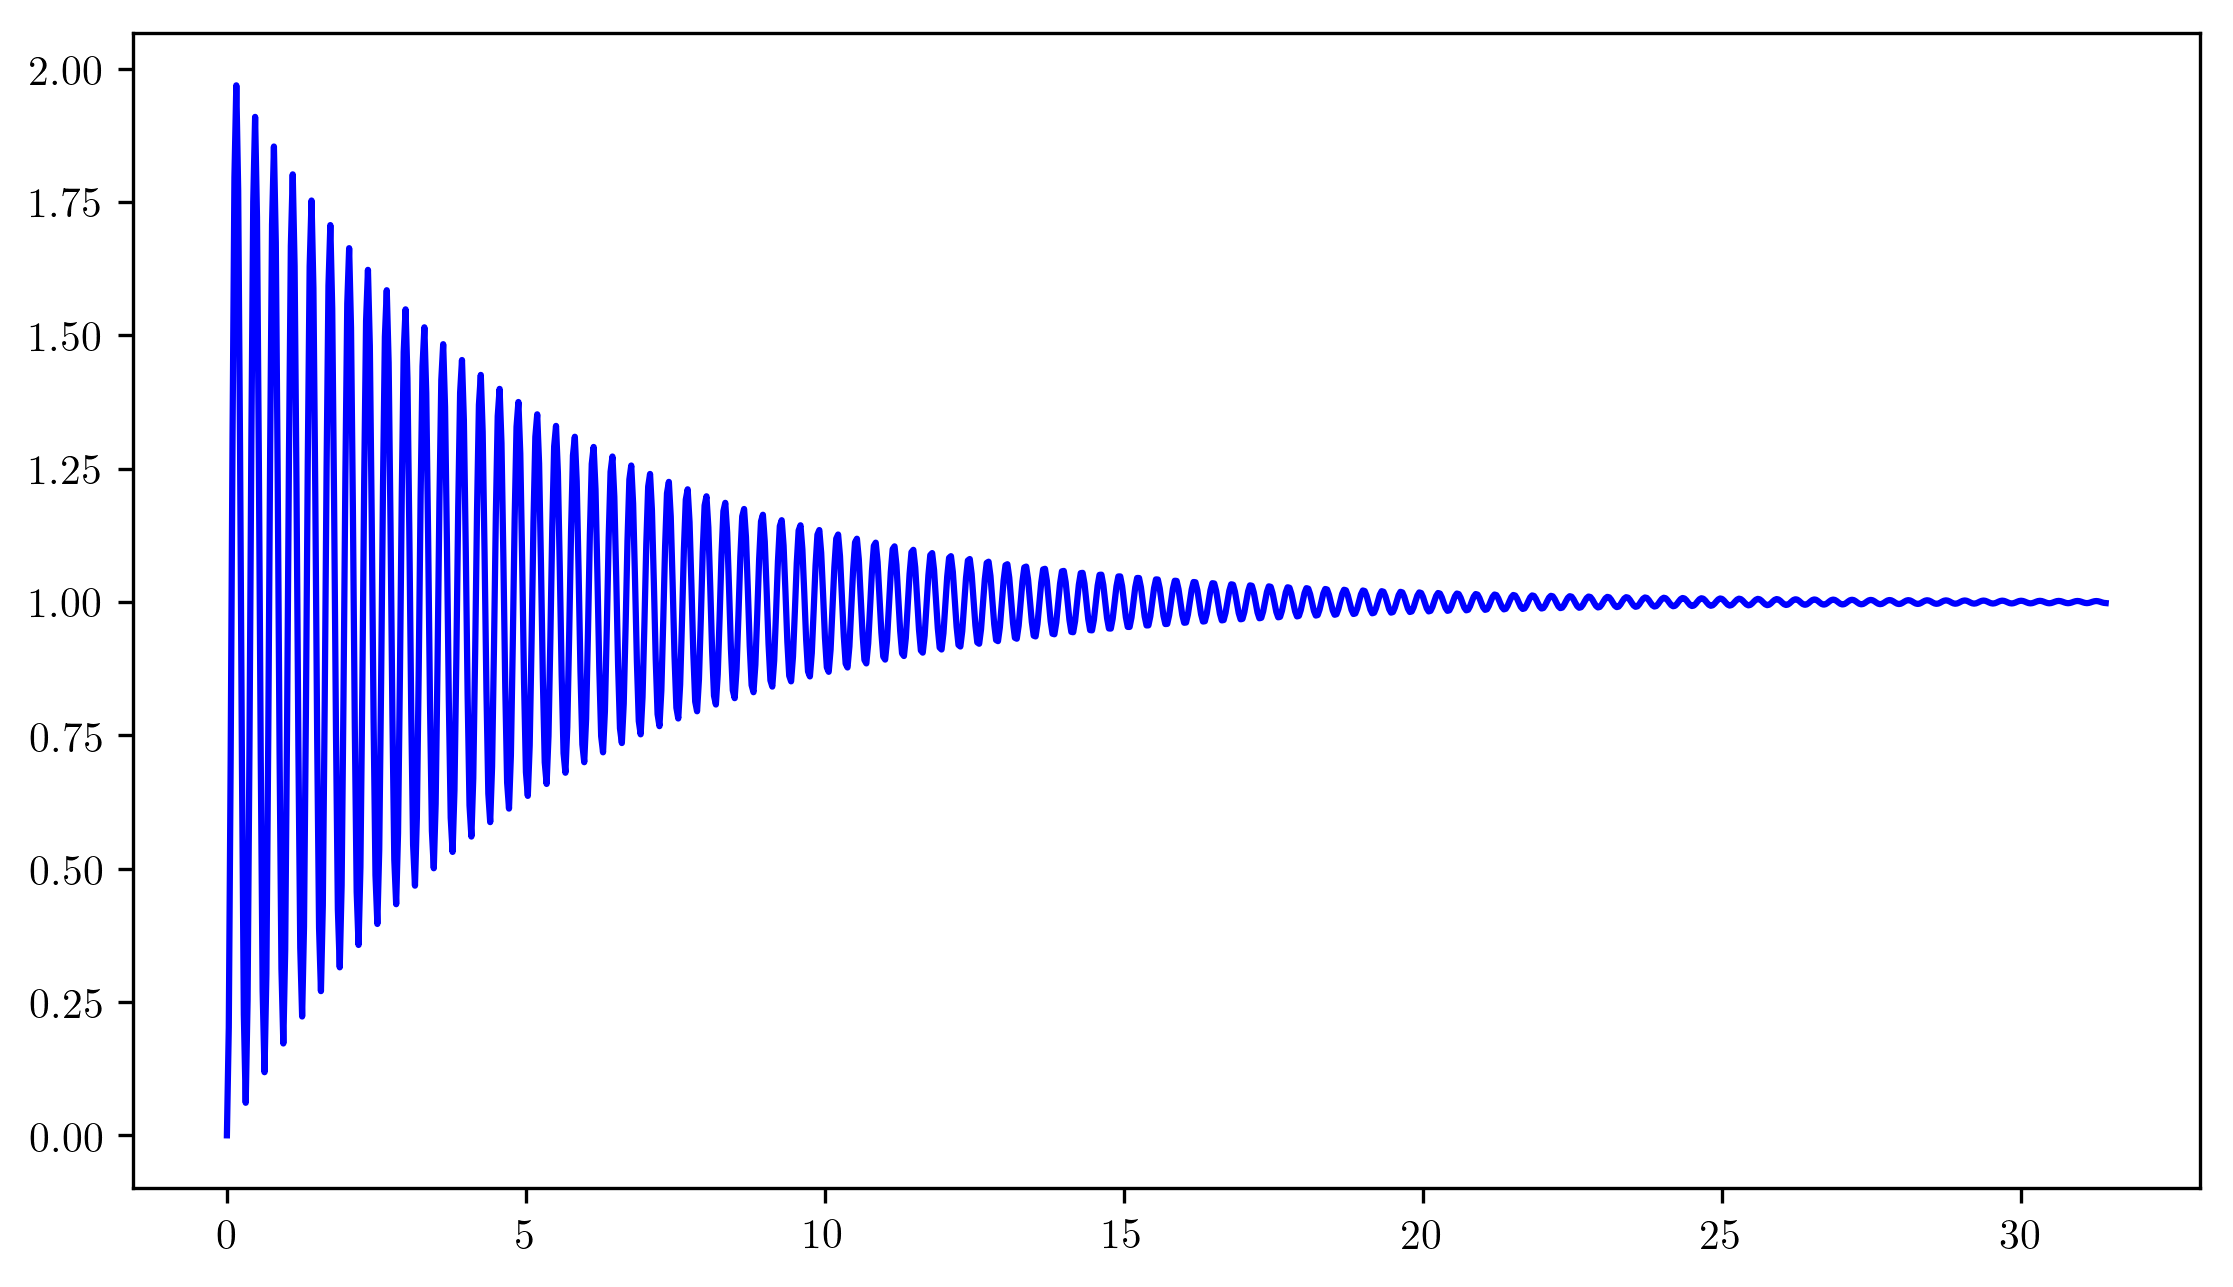
\includegraphics[width=\textwidth]{plusangle.png}
	\caption{$\Re[c(t)] - 0.1, \Im[c(t)] + 10$.}
	\label{fig:plusangle}
\end{figure}

\paragraph{Explain} The observation agrees with the prediction.

\clearpage
\item \textbf{Increased real part}

\paragraph{Predict} Only the real part is changed. Increasing it will cause the envelope to decay slower.

\begin{figure}[!h]
	\centering
	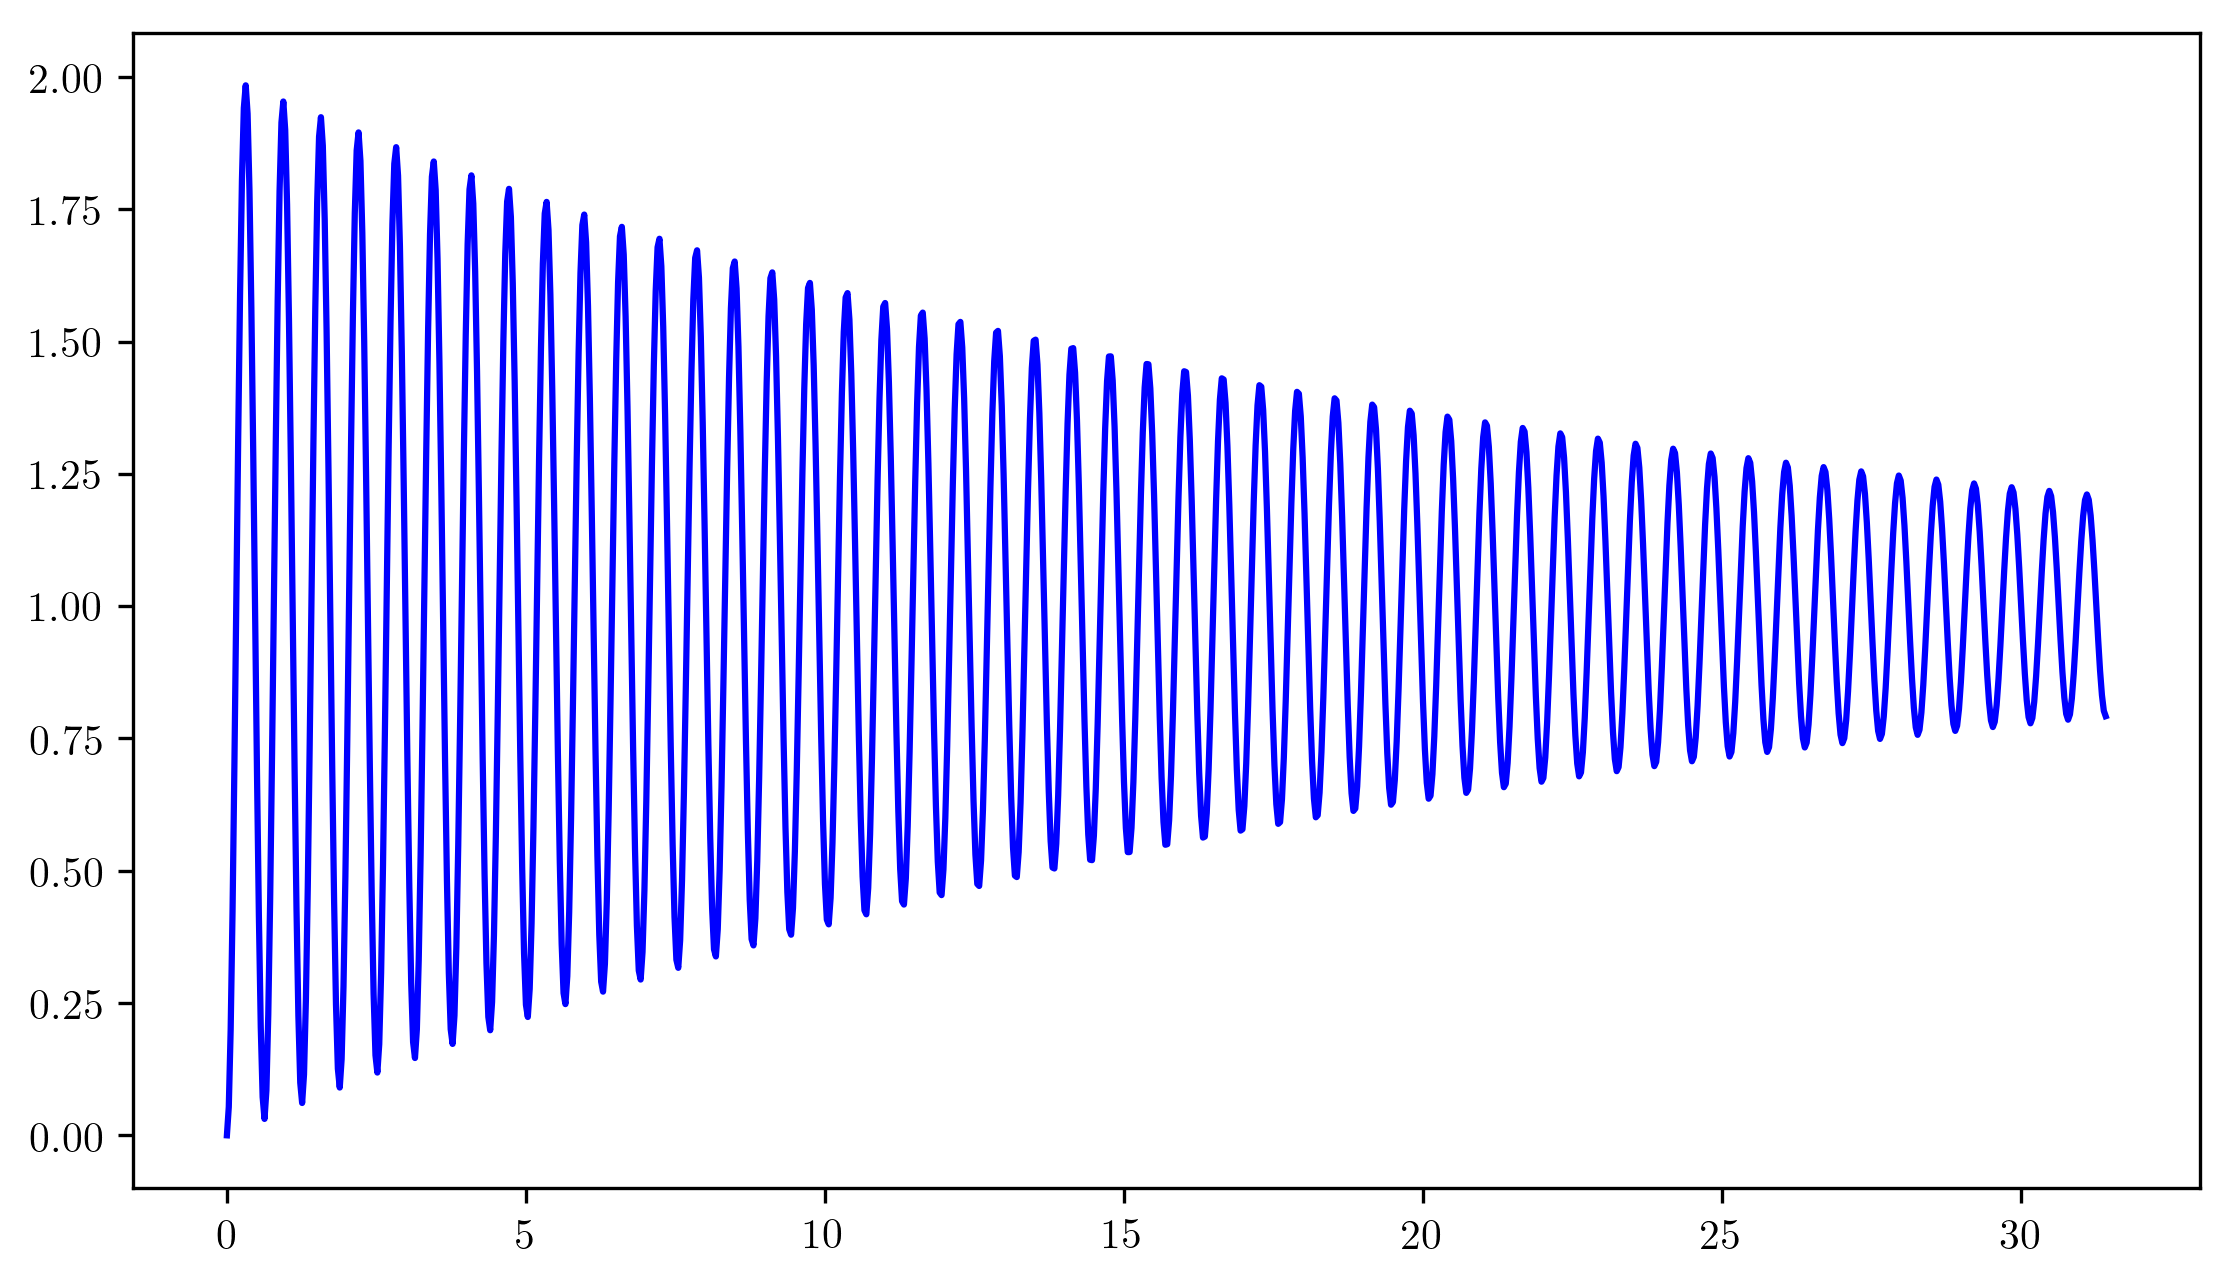
\includegraphics[width=\textwidth]{plusreal.png}
	\caption{$\Re[c(t)] + 0.05$.}
	\label{fig:plusreal}
\end{figure}

\paragraph{Explain} The observation agrees with the prediction.

\clearpage
\item \textbf{Narrow imaginary part}

\paragraph{Predict} Similar to the explanation for widening the imaginary part, narrowing it will decrease the frequency.

\begin{figure}[!h]
	\centering
	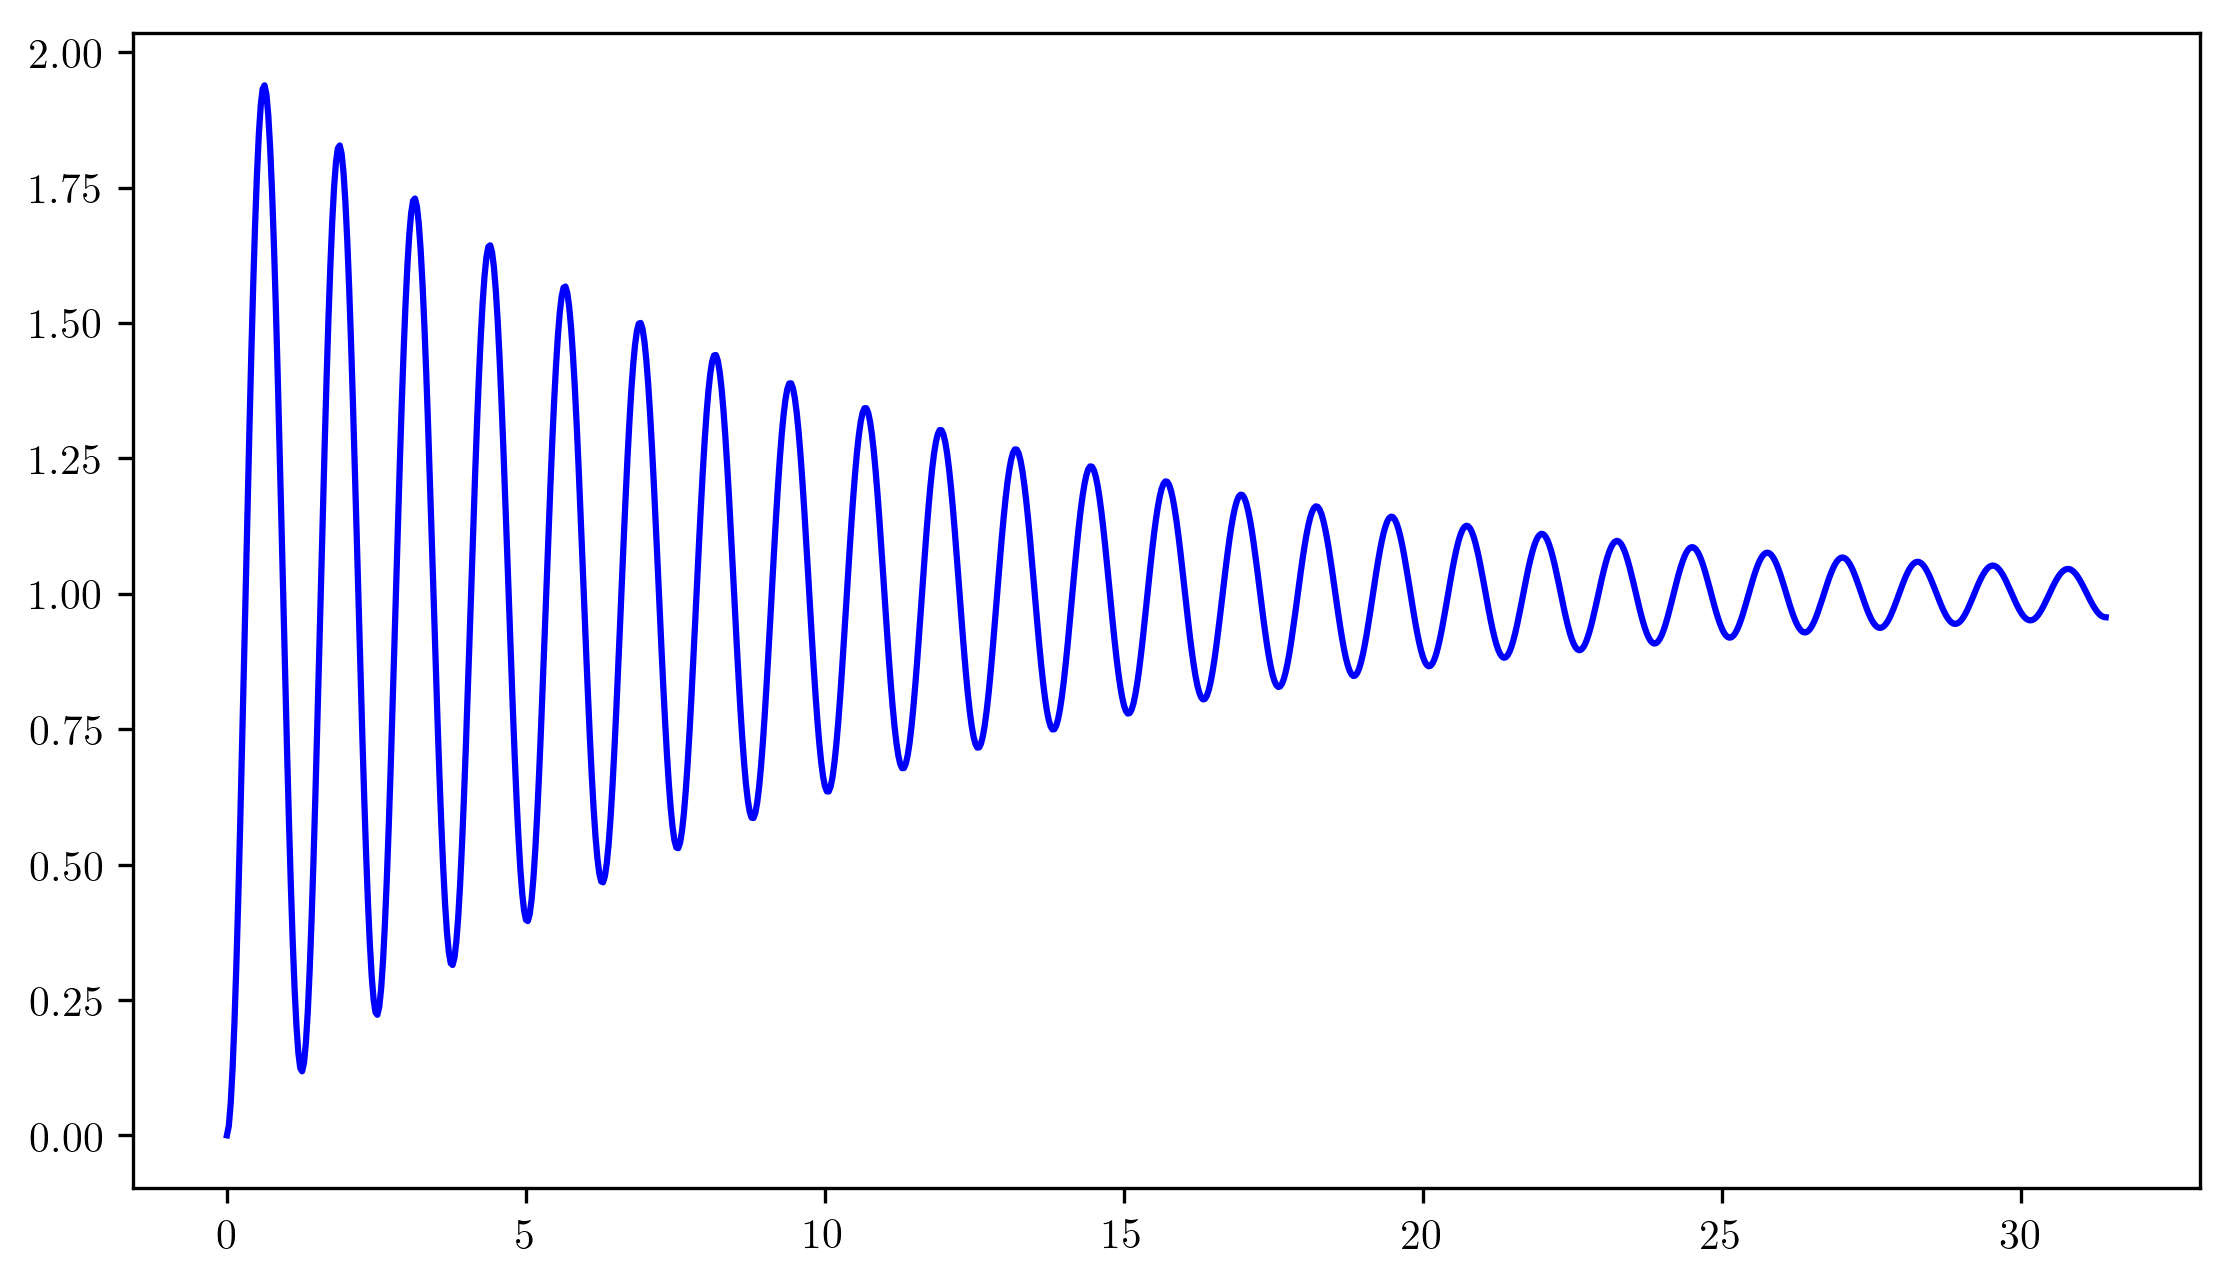
\includegraphics[width=\textwidth]{minusimag.png}
	\caption{$\Im[c(t)] - 5$.}
	\label{fig:minusimag}
\end{figure}

\paragraph{Explain} The observation agrees with the prediction.

\clearpage
\item \textbf{Much increased real part}

\paragraph{Predict} Greatly increasing the real part will greatly slow the decay of the envelope. The output will appear like a sinusoid with constant amplitude.

\begin{figure}[!h]
	\centering
	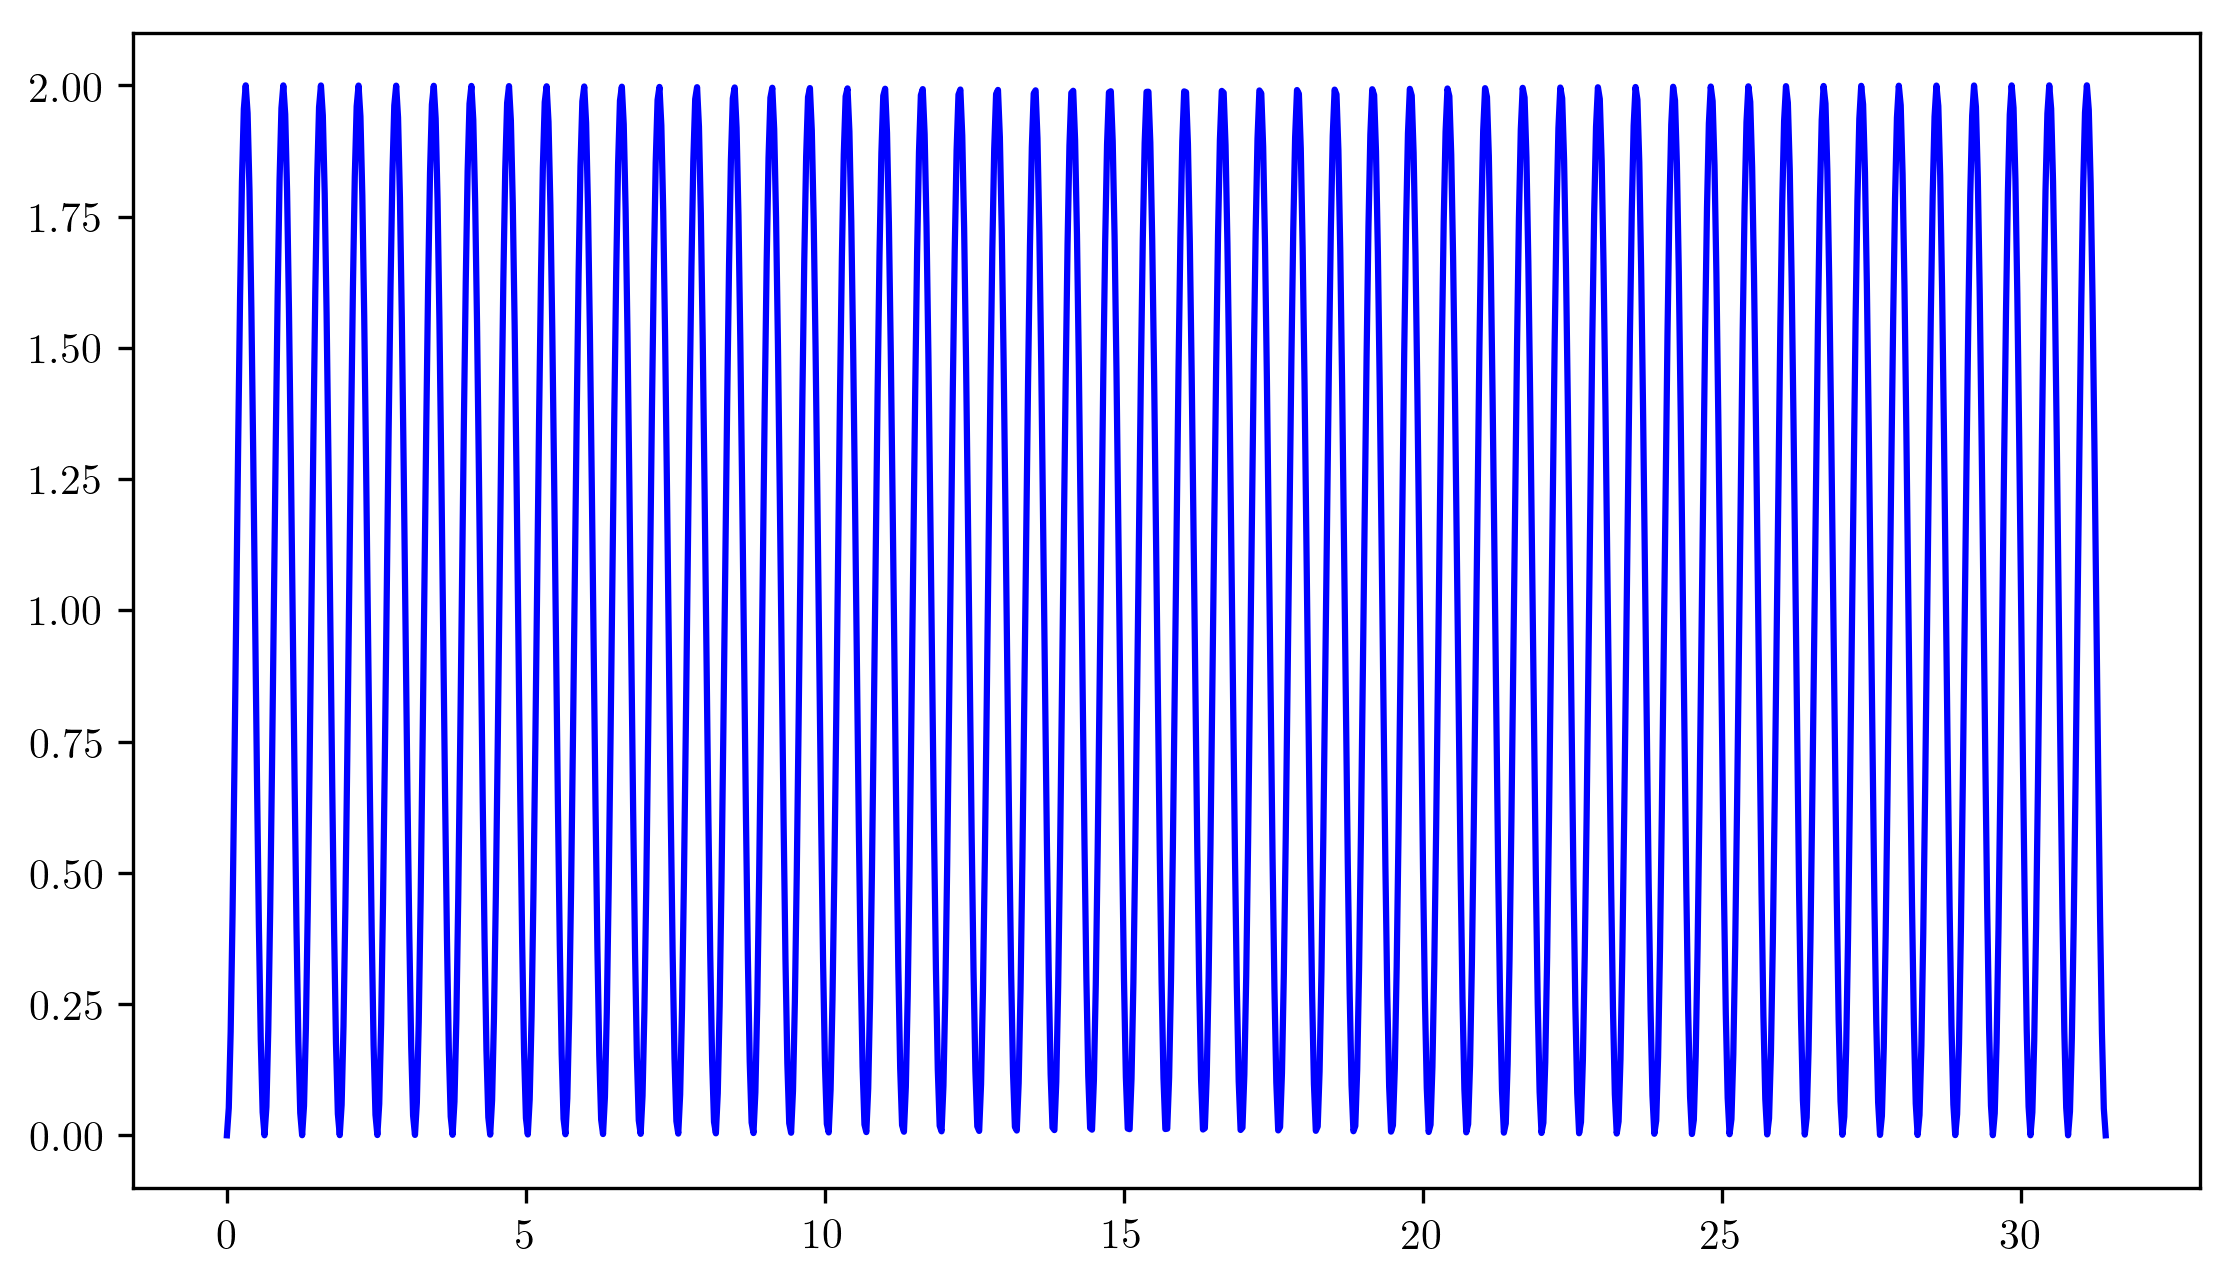
\includegraphics[width=\textwidth]{plusplusreal.png}
	\caption{$\Re[c(t)] + 0.1$.}
	\label{fig:plusimag}
\end{figure}

\paragraph{Explain} The observation agrees with the prediction.

\end{enumerate}

%\bibliographystyle{spp-bst}
%\bibliography{bibfile}

%\raggedbottom

%\pagebreak
%\pagebreak[3]
\iffalse
\newpage

\renewcommand\thefigure{A\arabic{figure}} 
\setcounter{figure}{0}
\fi %removing this will break the code for some reason

\end{document}

